%TOASK
%---------------------------------------------------------------------
%   documentclass
%---------------------------------------------------------------------
\documentclass[]{beamer}
% Class options include: notes, notesonly, handout, trans,
%                        hidesubsections, shadesubsections,
%                        inrow, blue, elcon-clr, grey, brown

%---------------------------------------------------------------------
%   packages
%---------------------------------------------------------------------
% Theme for beamer presentation.
\usepackage{beamerthemesplit}
% Other themes include: beamerthemebars, beamerthemelined,
%                       beamerthemetree, beamerthemetreebars
\usepackage[english]{babel}
\usepackage[enc=cp1250]{hrlatex}
\usepackage[T1]{fontenc} %pekne makcene
\usepackage{lmodern} %spolu s T1 smooth font!
\usepackage{cite} %bibtex
\usepackage[numbers]{natbib}
\usepackage{color} %for \textcolor{declared-color}{text}
\usepackage{floatflt} %to have tables and text beside
\usepackage{colortbl} %for \rowcolor command
\usepackage{scalefnt} %for scale font
\usepackage{pifont} %for ticks (check symbols)
\usepackage{pgfplots}
\usepackage{xcolor} %for \colorlet
\usepackage{lipsum}
\usepackage{bm}

\usepackage{tikz}
\usetikzlibrary{decorations.pathreplacing}
\usetikzlibrary{shapes,fit,calc,shadows,plotmarks}

\colorlet{city-clr}{green!70!black}
\colorlet{elcon-clr}{red}
\colorlet{event-clr}{blue}
\colorlet{waiting-clr}{olive}
\colorlet{cmt-clr}{gray}
\colorlet{oracle-clr}{orange!30}
\colorlet{cmt-clr}{gray}
\colorlet{oracle-clr}{orange!30}
\colorlet{algsec-clr}{black!50!red}

%---------------------------------------------------------------------
%   settings
%---------------------------------------------------------------------
\graphicspath{{./pics/}} %picture dir

\definecolor{tablehead}{RGB}{238,233,233} %nice smooth grey

\def\Tiny{ \font\Tinyfont = cmr10 at 3pt \relax  \Tinyfont}

\pgfrealjobname{presentation} % <-- NOTE: this needs to be the real document's basename
                        %     (else you'll only get an empty output file)

\newif\iffull
\fullfalse

\newif\iffinal % introduce a switch for draft vs. final document
\finaltrue % use this to compile the final document
\iffinal
  \newcommand{\inputTikZ}[1]{%
    \input{#1.tikz}%
  }
\else
  \newcommand{\inputTikZ}[1]{%
    \beginpgfgraphicnamed{#1-external}%
    \input{#1.tikz}%
    \endpgfgraphicnamed%
  }
\fi

%---------------------------------------------------------------------
%   environments
%---------------------------------------------------------------------
%\newcommand{\newblock}{}

\newcommand{\tick}{\ding{52}}
\newcommand{\cross}{\ding{55}}

%---------------------------------------------------------------------
%   theme
%---------------------------------------------------------------------
\usetheme{Darmstadt}
\usecolortheme{seahorse}

%---------------------------------------------------------------------
%   data
%---------------------------------------------------------------------
\title{\textbf{Distance oracles for timetable graphs}}
\subtitle{Di�tan�n� or�kula pre grafy reprezentuj�ce cestovn� poriadky}
\author{\textbf{Franti�ek Hajnovi�}}
\institute{FMFI UK}
\date{\today}

%---------------------------------------------------------------------
%   document
%---------------------------------------------------------------------
\begin{document}

	%---------------------------------------------------------------------
	%   Title page
	%---------------------------------------------------------------------
	{
    \setbeamertemplate{background canvas}{
        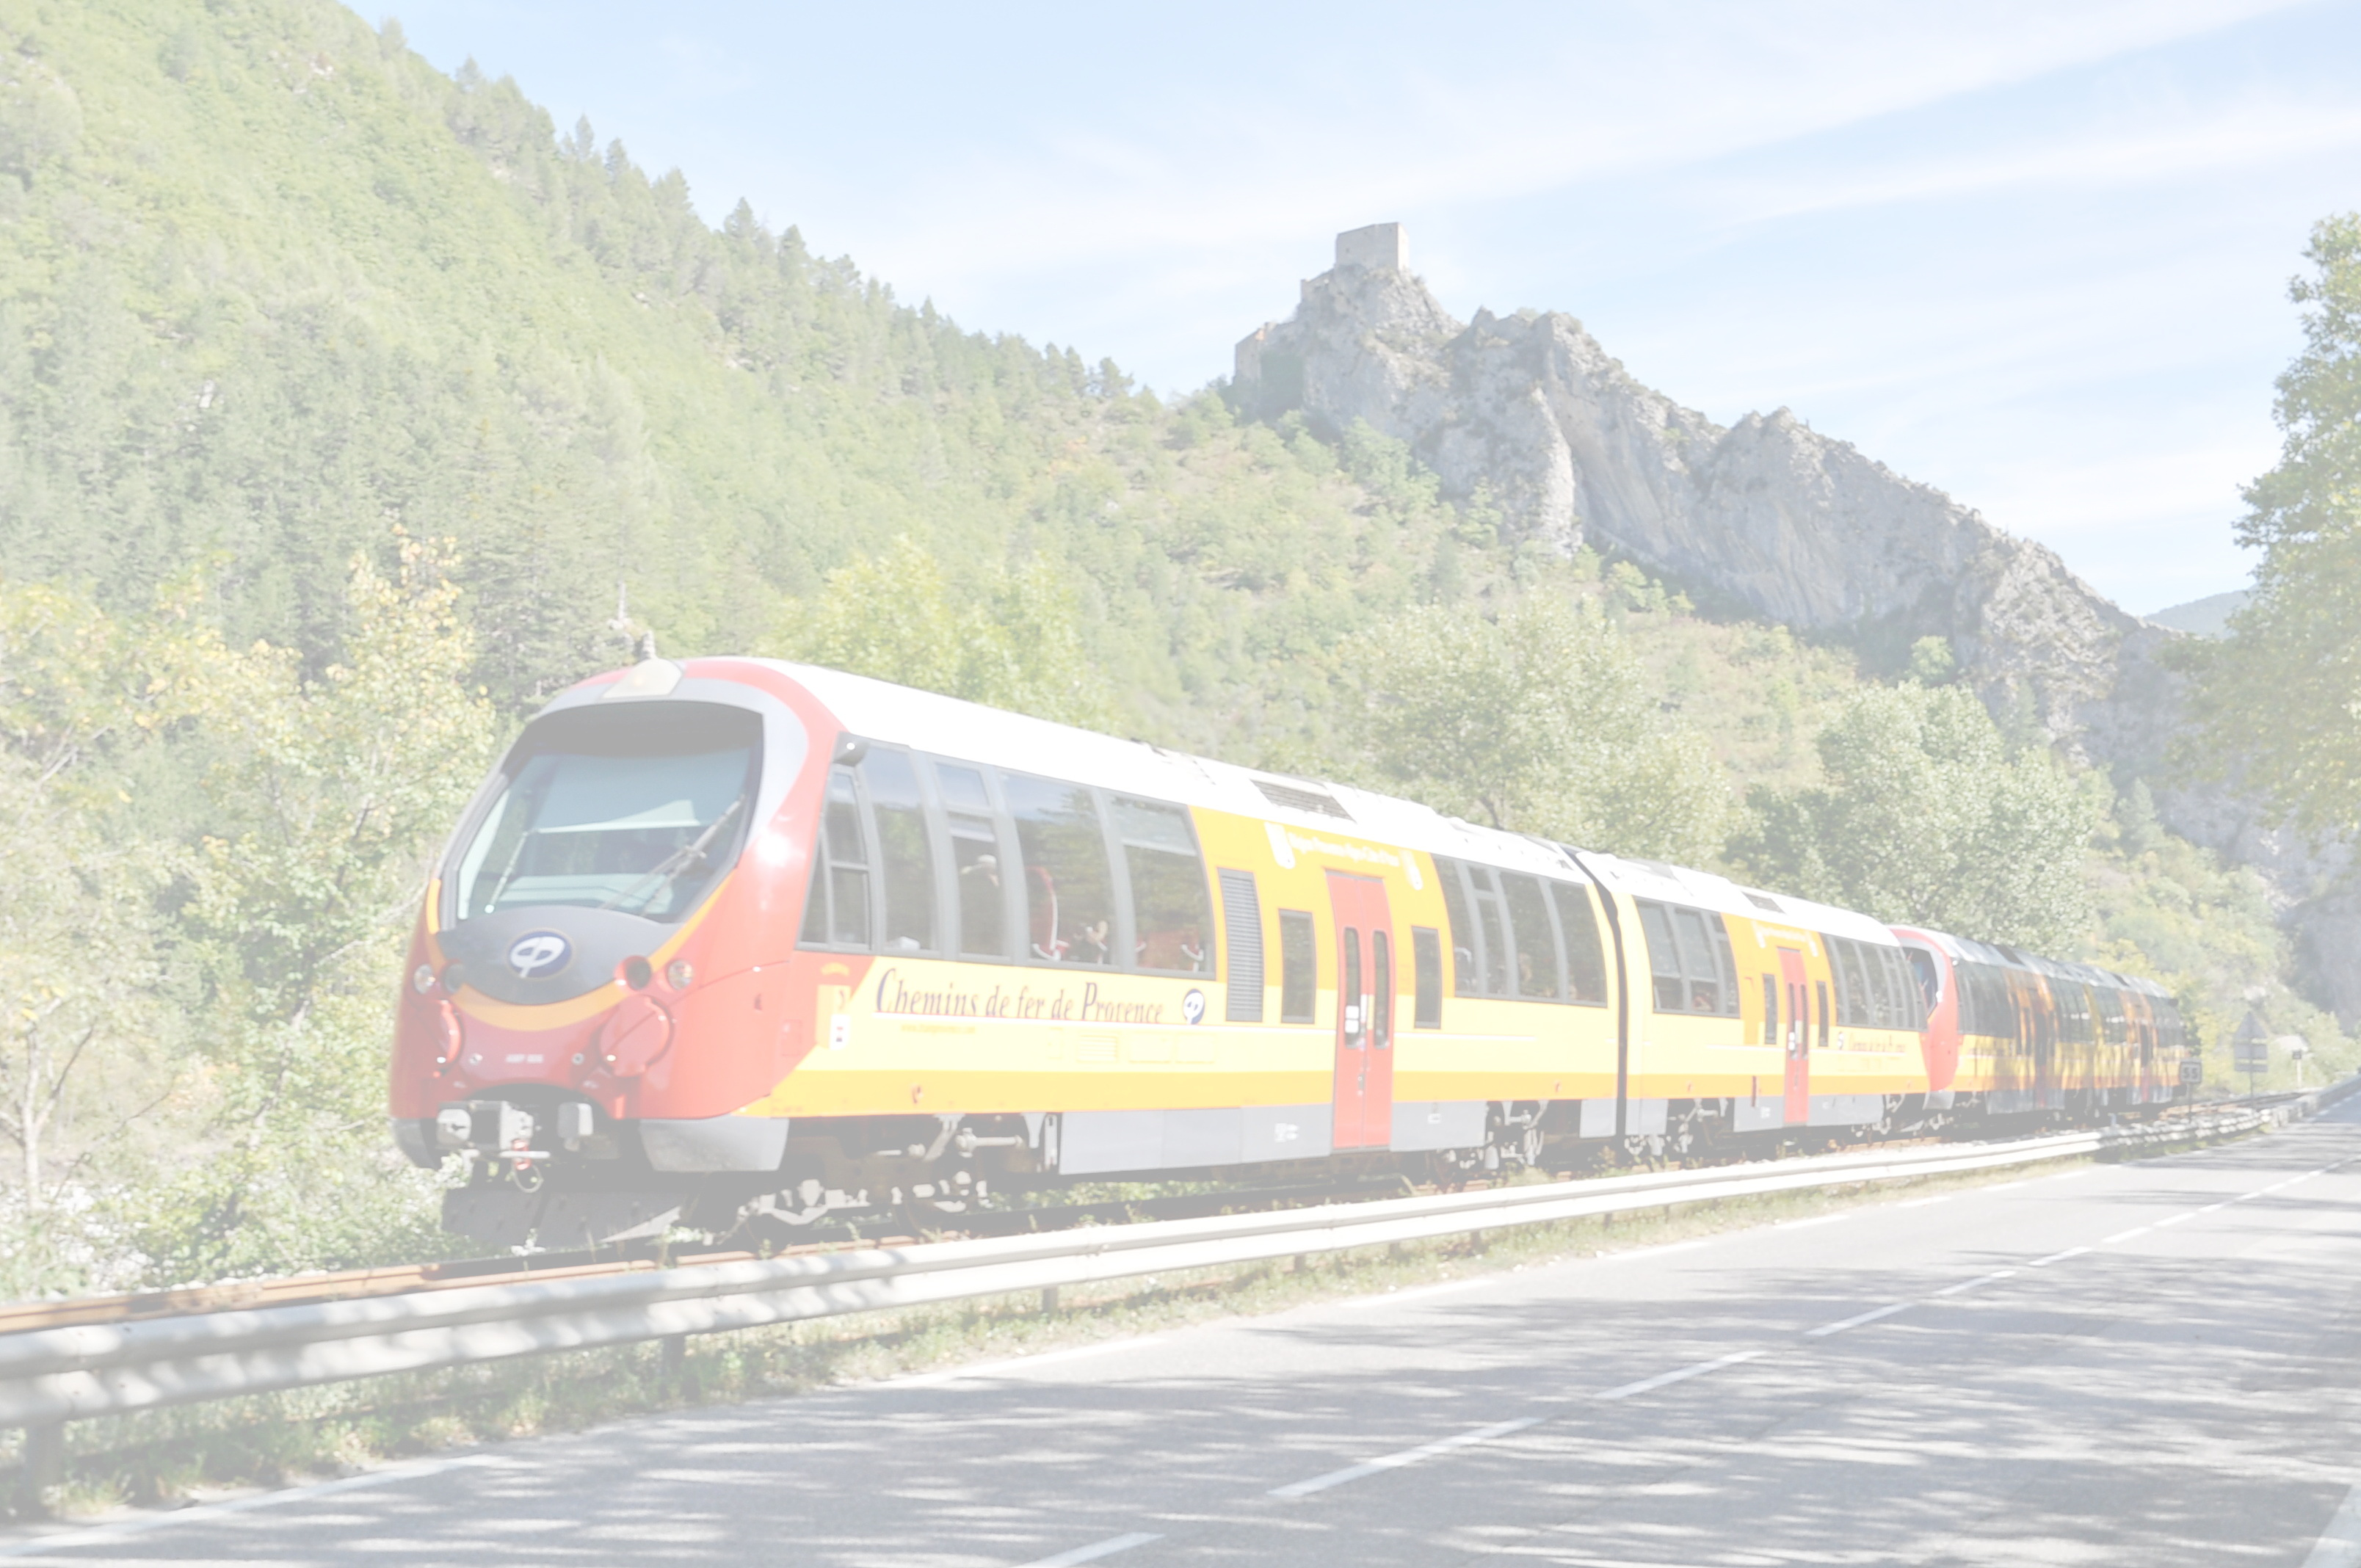
\includegraphics[height=\paperheight]{train.jpg}
    }
    \begin{frame}
        \titlepage
        \begin{center}
            Supervisor: \textit{doc. RNDr.} Rastislav Kr�lovi� \textit{PhD.}
        \end{center}
    \end{frame}
    }

	%---------------------------------------------------------------------
	%   Content
	%---------------------------------------------------------------------
    \begin{frame}
        \frametitle{Content}
        \tableofcontents
    \end{frame}

	%---------------------------------------------------------------------
	%   Introduction
	%---------------------------------------------------------------------
    \setbeamercolor{frametitle}{fg=elcon-clr!80!black}
    \section{Introduction}
    \begin{frame}
        \frametitle{Introduction}
        \begin{center}
            \textcolor{elcon-clr!80!black}{\textbf{Introduction}}
        \end{center}
    \end{frame}
    \setbeamercolor{frametitle}{fg=black!70}

		%---------------------------------------------------------------------
		%   What is it about?
		%---------------------------------------------------------------------
	    \begin{frame}
	        \frametitle{What is it about?}
	        \begin{itemize}
	            \item Given a timetable, we query - $(a, t, b)$ - for
	            \begin{itemize}
	            	\item \textbf{Earliest arrival} (EA) - $\bm{t_{(a, t, b)}^{*}}$
	            	\item \textbf{Optimal connection} (OC) - $\bm{c_{(a, t, b)}^{*}}$
	            \end{itemize}
	        \end{itemize}
	        \vspace{-0.5cm}
	        \begin{figure}[h!]
				\scriptsize
                \begin{center}
					\inputTikZ{./tikzpics/connection}
                \end{center}
            \end{figure}
            \vspace{-0.5cm}	
            \begin{itemize}
            	\item<2> Motivation: large-scale timetable search engines (\emph{cp.sk, imhd.sk}...)
				\item<2> Approach: (distance) oracle-based approach~\cite{apxdo05} - pre-computation
			\end{itemize}
			\vspace{-0.5cm}
			\uncover<2>{\begin{figure}[h!]
                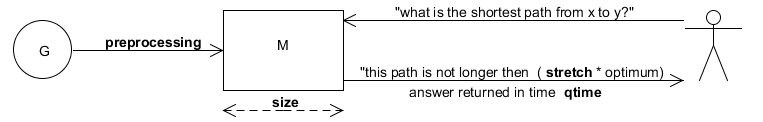
\includegraphics[height=0.5in]{dodiagram.png}
            \end{figure}}
	    \end{frame}
	    
	    %---------------------------------------------------------------------
        %   TT and UG graph
        %---------------------------------------------------------------------
        \begin{frame}
            \frametitle{Timetable and underlying graph}        
	        \begin{columns}[c]
            \column{2.7in}
				\begin{table}{
	                \scriptsize
	                \begin{tabular}{c|c|c|c}
	                %legend
	                    \hline
	                    \rowcolor{tablehead}
	                    \multicolumn{2}{>{\columncolor{tablehead}}c|}{\textbf{Place}} & \multicolumn{2}{>{\columncolor{tablehead}}c}{\textbf{Time}} \\
						\hline
	                    \rowcolor{tablehead}
	                    \textbf{From} & \textbf{To} & \textbf{Departure} & \textbf{Arrival} \\
	                %data
						\hline
	                    \textcolor{city-clr}{A} & \textcolor{city-clr}{B} & 10:00 & 10:45 \\
						\textcolor{city-clr}{B} & \textcolor{city-clr}{C} & 11:00 & 11:30 \\
						\textcolor{city-clr}{B} & \textcolor{city-clr}{C} & 11:30 & 12:10 \\
						\textcolor{city-clr}{B} & \textcolor{city-clr}{A} & 11:20 & 12:30 \\
						\textcolor{city-clr}{C} & \textcolor{city-clr}{A} & 11:45 & 12:15 \\
					\end{tabular}}
					\caption{\textbf{Timetable} - a set of \textbf{elementary connections} (between pairs of \textbf{\textcolor{city-clr}{cities}})}
	            	\normalsize
				\end{table}
            \column{2.3in}
            	\begin{figure}[h!]
					\scriptsize
	                \begin{center}
						\inputTikZ{./tikzpics/ug}
	                \end{center}
                    \caption{\textbf{Underlying graph}}
                \end{figure}
			\end{columns}
			\begin{itemize}
				\item<2> Goals:
				\begin{itemize}
	                \item<2> Devise methods to tackle EA/OC problem
		            \item<2> Analyse properties of real-world timetables
	            \end{itemize}			
			\end{itemize}
		\end{frame}
		
	%---------------------------------------------------------------------
	%   Contribution 
	%---------------------------------------------------------------------
    \setbeamercolor{frametitle}{fg=elcon-clr!80!black}
    \section{Contribution}
    \begin{frame}
        \frametitle{Contribution}
        \begin{center}
            \textcolor{elcon-clr!80!black}{\textbf{Contribution}}
        \end{center}
    \end{frame}
    \setbeamercolor{frametitle}{fg=black!70}

	    %---------------------------------------------------------------------
        %   Idea
        %---------------------------------------------------------------------
        \subsection{Underlying shortest paths}
        \begin{frame}
            \frametitle{Idea}
			\begin{itemize}
                \item \textit{``Usually we go through the same sequence of cities''}
            \end{itemize}
            \vspace{0.5cm}
            \begin{columns}[c]
            \column{2.7in}
            	\vspace{-1cm}
	            \begin{figure}[h]
					\scriptsize
	                \begin{center}
	                    \inputTikZ{./tikzpics/pathfunc}
	                \end{center}
	            \end{figure}
	            \vspace{-0.7cm}
	            \begin{itemize}
	            	\small
	            	\item $p$ is \textbf{USP} $\iff$ $\exists t: path(c_{(a, t, b)}^{*}) = p$
	            	\item we have USP $p$: $expand(p)$ $\rightarrow$ $c_{(a, t, b)}^{*}$
	            	\item<2-> \textbf{Overtaking}~\cite{timetablemodelsalgs07} causes problems, but can be easily removed
	            \end{itemize}
	        \column{2.3in}
		        \vspace{-0.5cm}
	        	\begin{figure}[h!]
	                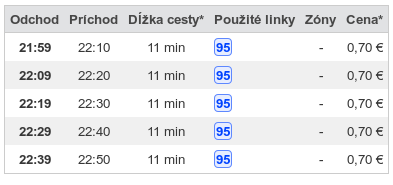
\includegraphics[height=0.9in]{redundancy.png}
	            \end{figure}
	            \uncover<2->{
	            	\vspace{-0.5cm}
	            	\begin{table}{
	                \tiny
	                \begin{tabular}{c|c}
	                %legend
	                    \hline
	                    \rowcolor{tablehead}
	                    \textbf{Name} & \textbf{Overtaken edges (\%)} \\
	                %data
						\hline
						\textit{air01} & 1\% \\
						\textit{cpru} & 2\% \\
						\textit{cpza} & 2\% \\
						\textit{montr} & 1\% \\
						\textit{sncf} & 2\% \\
						\textit{sncf-ter} & 2\% \\
						\textit{sncf-inter} & 8\% \\
						\textit{zsr} & 0\% \\
					\end{tabular}}
	            	\normalsize
				\end{table}}
			\end{columns}
        \end{frame}
        
        %---------------------------------------------------------------------
        %   USP-OR
        %---------------------------------------------------------------------
        \subsection{USP-OR}
        \begin{frame}
            \frametitle{\textit{USP-OR}}
            \begin{columns}[c]
            \column{2.4in}
				\begin{itemize}
					\small
					\item<1-> Pre-compute \textit{all conn.} - space $\mathcal{O}(h \; n^{2} \gamma)$
					\begin{itemize}
						\item $\bm{\gamma}$ - the average OC size
	                	\item daily height usually $200$ < $h$ < $800$
	                \end{itemize}
	                \item<2-> Pre-compute \textit{all USPs} - space $\mathcal{O}(\tau \; n^{2} \gamma)$
	                \begin{itemize}
	                	\item $\bm{\tau(x, y)}$ - \# of USPs between $x$ and $y$
	                \end{itemize}
				\end{itemize}
	        \column{2.6in}
	        	\uncover<2->{\begin{table}{
	                \scriptsize
	                \begin{tabular}{c|c|c|c}
	                %legend
	                    \hline
	                    \rowcolor{tablehead}
	                    \textbf{Name} & \textbf{avg $\bm{\tau}$} & \textbf{max $\bm{\tau(x, y)}$} & \textbf{$\bm{\gamma}$} \\
	                %data
						\hline
						\textit{air01} & 5.8 & 30 & 3.0 \\
						\textit{cpru} & 7.0 & 64 & 13.8 \\
						\textit{cpza} & 5.1 & 42 & 11.1 \\
						\textit{montr} & 4.3 & 30 & 20.3 \\
						\textit{sncf} & 4.3 & 24 & 10.5 \\
						\textit{sncf-inter} & 0.6 & 19 & 7.9 \\
						\textit{sncf-ter} & 6.1 & 33 & 10.8 \\
						\textit{zsr} & 2.5 & 19 & 13.7 \\
					\end{tabular}}
					\caption{\footnotesize Daily, 200 station timetables}
	            	\normalsize
				\end{table}}
	        \end{columns}
	        \vspace{-0.5cm}
	        \makebox[\linewidth]{\parbox{12cm}{
	        \uncover<2->{\begin{table}[h!]
	        	\scriptsize
				\centering
				\begin{tabular}{l|c|c|c|c}
				%legend
					\cellcolor{oracle-clr} \textit{\textbf{USP-OR}} & \cellcolor{oracle-clr} $\bm{prep}$ & \cellcolor{oracle-clr} $\bm{size}$ & \cellcolor{oracle-clr} $\bm{qtime}$ & \cellcolor{oracle-clr} $\bm{stretch}$ \\
				%data
					\hline
					\cellcolor{oracle-clr} \textbf{guaranteed} & $\mathcal{O}(hn^{2} (\log n + \delta))$ & $\mathcal{O}(\tau n^{2} \gamma)$ & avg. $\mathcal{O}(\tau \gamma)$ & $1$ \\
					\cellcolor{oracle-clr} \textbf{$\bm{\tau}$ const., $\bm{\gamma \leq \sqrt{n}}$, $\bm{\delta \leq \log n}$} & $\mathcal{O}(hn^{2} \log n)$ & $\mathcal{O}(n^{2.5})$ & avg. $\mathcal{O}(\sqrt{n})$ & $1$ \\
				\end{tabular}
				\caption{$\delta$ - the UG density $\frac{m}{n}$}
			\end{table}}
			}}
			\vspace{-0.7cm}
			\begin{itemize}
				\item<3-> Space $\mathcal{O}(n^{2.5})$ too big anyway
			\end{itemize}
        \end{frame}
        
        %---------------------------------------------------------------------
        %   USP-OR - grafy
        %---------------------------------------------------------------------
        \begin{frame}
            \frametitle{\textit{USP-OR} - $\tau$ evolution}
            \begin{columns}[c]
            \column{2.4in}
				\begin{figure}[h]
					\scriptsize
	                \begin{center}
	                    \inputTikZ{./tikzpics/plot_usp_air01_timerange}
	                \end{center}
	                \caption{\footnotesize Changing of $\tau$ with increased time range in \textit{air01} dataset. 1 day = about 800 in height}
	            \end{figure}
	        \column{2.4in}
	        	\begin{figure}[h]
					\scriptsize
	                \begin{center}
	                    \inputTikZ{./tikzpics/plot_usp_sncf_size}
	                \end{center}
	                \caption{\footnotesize Changing of $\tau$ with increased \# of stations in \textit{sncf} dataset}
	            \end{figure}
	        \end{columns}
        \end{frame}
        
        %---------------------------------------------------------------------
        %   USP-OR-A
        %---------------------------------------------------------------------
        \subsection{USP-OR-A}
        \begin{frame}
            \frametitle{\textit{USP-OR-A}}
		    \footnotesize
			\begin{itemize}
				\item Pre-compute USPs only among \textit{some} cities in UG: $\bm{(r_{1}, r_{2}, r_{3})}$ \textbf{access node set}
				\begin{itemize}
					\footnotesize
					\item Small size: $|\mathcal{A}| \leq r_{1} \cdot \sqrt{n}$
					\item Small node neighbourhoods: $avg \; (|neigh(x)|)^{2} \leq r_{2} \cdot n$
					\item Few local access nodes: $|lan_{\mathcal{A}}(x)| \leq r_{3}$
				\end{itemize}
	        \end{itemize}
	        \vspace{-0.2cm}
	        \makebox[\linewidth]{\parbox{12cm}{\begin{figure}[h]
				\scriptsize
                \begin{center}
					\inputTikZ{./tikzpics/uspora}
                \end{center}
            \end{figure}
            }}
        \end{frame} 
        
		%---------------------------------------------------------------------
        %   USP-OR-A and ANs
        %---------------------------------------------------------------------        
        \begin{frame}
            \frametitle{\textit{USP-OR-A} and access nodes}
		    \makebox[\linewidth]{\parbox{12cm}{\begin{table}[h!]
				\centering
				\tiny
				\begin{tabular}{l|c|c}
				%legend
					\cellcolor{oracle-clr} \textit{\textbf{USP-OR-A}} & 
					\cellcolor{oracle-clr} \textbf{guaranteed} & 
					\cellcolor{oracle-clr} \textbf{$\bm{\tau, r_{1}, r_{2}, r_{3}}$ const., $\bm{\gamma \leq \sqrt{n}}$, $\bm{\delta \leq \log n}$} \\
				%data
					\hline
					\cellcolor{oracle-clr} $\bm{prep}$ & $\mathcal{O}(f(n) + (r_{1} + r_{2}) (\delta + \log n) h n^{1.5})$ & $\mathcal{O}(f(n) + h n^{1.5} \log n)$ \\
					\cellcolor{oracle-clr} $\bm{size}$ & $\mathcal{O}(r_{2} n^{1.5} + r_{1}^{2} \tau_{\mathcal{A}} \gamma_{\mathcal{A}} n)$ & $\mathcal{O}(n^{1.5})$ \\
					\cellcolor{oracle-clr} $\bm{qtime}$ & avg. $\mathcal{O}(r_{2} r_{3} \sqrt{n} (\log (r_{2}n) + \delta) + r_{3}^{2} \tau_{\mathcal{A}} \gamma_{\mathcal{A}})$ & avg. $\mathcal{O}(\sqrt{n} \log n)$ \\
					\cellcolor{oracle-clr} $\bm{stretch}$ & $1$ & $1$ \\
				\end{tabular}
			\end{table}
			}}
			\vspace{-0.5cm}
			\begin{itemize}
				\small
				\item Much depends on choosing good AN set
				\item<2-> Minimize $|\mathcal{A}|$ s.t. $\forall x: |neigh_{\mathcal{A}}(x)| \leq \sqrt{n}$ $\rightarrow$ NP-complete
				\item<2-> Choose ANs based on degree/betweenness centrality
			\end{itemize}
			\vspace{-0.2cm}
			\uncover<2->{\begin{columns}[c]
            \column{2.4in}
            	\begin{figure}[h]
					\scriptsize
	                \begin{center}
	                    \inputTikZ{./tikzpics/plot_hbcdeg_sncf_size}
	                \end{center}
	                \vspace{-0.3cm}
	                \caption{\scriptsize $|\mathcal{A}| = r_{1} \sqrt{n} \approx r_{1} 51$ (\textit{sncf}).}
	            \end{figure}
	        \column{2.4in}
	        	\begin{figure}[h]
					\scriptsize
	                \begin{center}
	                    \inputTikZ{./tikzpics/plot_hbcdeg_cpru_size}
	                \end{center}
	                \vspace{-0.3cm}
	                \caption{\scriptsize $|\mathcal{A}| = r_{1} \sqrt{n} \approx r_{1} 30$ (\textit{cpru}).}
	            \end{figure}
	        \end{columns}
	        }
        \end{frame} 
        
        %---------------------------------------------------------------------
        %   Locsep
        %---------------------------------------------------------------------
        \begin{frame}
            \frametitle{\textit{Locsep}}
            \begin{itemize}
            	\item Select AN that locally separates many vertices
            \end{itemize}
            \begin{columns}[c]
            \column{2.5in}
	            \begin{figure}[h]
					\scriptsize
	                \begin{center}
						\inputTikZ{./tikzpics/locsep}
	                \end{center}
	            \end{figure}
	        \column{2.5in}
	        	\begin{figure}[h]
					\scriptsize
	                \begin{center}
	                    \inputTikZ{./tikzpics/plot_locsep_sncf_size}
	                \end{center}
	                \vspace{-0.3cm}
	                \caption{\scriptsize $|\mathcal{A}| = r_{1} \sqrt{n} \approx r_{1} 51$ (\textit{sncf}).}
	            \end{figure}
	        \end{columns}

        \end{frame}
        
		%---------------------------------------------------------------------
        %   Results and comparison
        %---------------------------------------------------------------------
        \subsection{Results and comparison}
        \begin{frame}
            \frametitle{Results}
            \begin{itemize}
            	\item Time-dependent Dijkstra's algorithm with Fibonacci heap priority queue $\mathcal{O}(m + n \log n)$
            \end{itemize}
			\begin{columns}[c]
            \column{2.4in}
				\begin{figure}[h]
					\scriptsize
	                \begin{center}
	                    \inputTikZ{./tikzpics/plot_usporall_sncf_size}
	                \end{center}
	                \caption{\footnotesize \textit{USP-OR-A} + \textit{Locsep} vs. \textit{USP-OR} vs. \textit{TD Dijkstra} on \textit{sncf} dataset. Changing $n$.}
	            \end{figure}
	        \column{2.4in}
	        	\begin{figure}[h]
					\scriptsize
	                \begin{center}
	                    \inputTikZ{./tikzpics/plot_usporall_zsr_trange}
	                \end{center}
	                \caption{\footnotesize \textit{USP-OR-A} + \textit{Locsep} vs. \textit{USP-OR} vs. \textit{TD Dijkstra} on \textit{zsr} dataset. Changing time range.}
	            \end{figure}
	        \end{columns}
        \end{frame}      
        
        %---------------------------------------------------------------------
        %   Existing methods
        %---------------------------------------------------------------------
        \begin{frame}
            \frametitle{Existing methods}
            \begin{columns}
			\column{2.4in}
				\begin{itemize}
					\item \textbf{Time-dependent SHARC} \cite{sharc08}, \textbf{Time-dependent CH} \cite{timedepch09}
					\begin{itemize}
						\item Speed-ups of about 26 / 1500, respectively (EA only)
						\item Meant for time-dependent routing in road networks
					\end{itemize}
					\item \textbf{Time-expanded approach} \cite{engtimeexp09}
				\end{itemize}	
	        \column{2.4in}
	        	\begin{table}{
					\scriptsize
		        	\centering
					\begin{tabular}{c|c|c}
					%legend
			            \rowcolor{tablehead}
			            \textbf{Name} & \textit{\textbf{USP-OR}} & \textit{\textbf{USP-OR-A}} \\
					%data
						\hline
						\textit{cpru} & 14.5 & 1.7 \\
						\textit{cpza} & 14.3 & 1.7 \\
						\textit{montr} & 8.8 & 1.5 \\
						\textit{sncf} & 64.8 & 5.4 \\
						\textit{sncf-inter} & 27.0 & 3.6 \\
						\textit{sncf-ter} & 78.3 & 6.3 \\
						\textit{zsr} (daily) & 19.3 & 2.14 \\
					\end{tabular}}
					\caption{\scriptsize Speed-up of \textit{USP-OR} and \textit{USP-OR-A} with \textit{Locsep}}
				\end{table}
	        \end{columns}
	        \vspace{-0.3cm}
	        \makebox[\linewidth]{\parbox{10.7cm}{
	        \begin{itemize}
	        	\small
				\item Max speed-up of 56 (Railways with 30000 stations!)
				\item Remodelling unimportant stations in TE graphs
			\end{itemize}
			}}
	        \makebox[\linewidth]{\parbox{12.3cm}{
			\begin{itemize}
				\item Theory vs. practice difference: transfers, cost of travel...
			\end{itemize}				       
			}} 
        \end{frame}            
      
        %---------------------------------------------------------------------
        %   NN
        %---------------------------------------------------------------------
        \subsection{Neural networks}
        \begin{frame}
            \frametitle{Neural network approaches}
			\begin{itemize}
				\small
				\item Multi-layer perceptron, back propagation
				\item Input layer = \textcolor{event-clr}{events} + \textcolor{city-clr}{cities}. 
				\item Output layer = arcs of UG $\rightarrow$ USP
			\end{itemize}
			\begin{figure}[h]
				\scriptsize
                \begin{center}
                    \inputTikZ{./tikzpics/neural}
                \end{center}
            \end{figure}
            \vspace{-0.5cm}
			\begin{columns}
			\column{2.4in}
				\begin{itemize}
					\item Tendency to remember USPs
					\item Long training times
				\end{itemize}  
	        \column{2.4in}
		        \begin{table}{
	                \tiny
	                \begin{tabular}{c|c|c|c}
	                %legend
	                    \hline
	                    \rowcolor{tablehead}
	                    \textbf{Name} & \textbf{Conn.} & \textbf{Found} & \textbf{Was optimum (\%)} \\
	                %data
						\hline
						air01 & 931 & 573 & 18.7\% \\
						cpru & 481 & 281 & 48\% \\
						montr & 527 & 346 & 86.7\% \\
						zsr & 672 & 307 & 76.2\% \\
					\end{tabular}}
					\caption{Timetables with 30 cities}
	            	\normalsize
				\end{table}
			\end{columns}
        \end{frame}  
    
    %---------------------------------------------------------------------
	%   Conclusion
	%---------------------------------------------------------------------
    \setbeamercolor{frametitle}{fg=elcon-clr!80!black}
    \section{Conclusion}
    \begin{frame}
        \frametitle{Conclusion}
        \begin{center}
            \textcolor{elcon-clr!80!black}{\textbf{Conclusion}}
        \end{center}
    \end{frame}
    \setbeamercolor{frametitle}{fg=black!70}
    
    	%---------------------------------------------------------------------
        %   Conclusion
        %---------------------------------------------------------------------
        \begin{frame}
            \frametitle{Conclusion}
			\begin{itemize}
				\item Trying out \textbf{novel approaches} to find optimal connections in timetables
				\begin{itemize}
					\item \textit{USP-OR}: Exact and very quick answers (speed-up $\approx$ 60) but high space
					\item \textit{USP-OR-A}: Exact and quick answers (speed-up $\approx$ 6) less space-consuming
					\item \textit{NN}: Problem too challenging for NN/try different types of network
				\end{itemize}
			\end{itemize}
			\begin{columns}
			\column{2.6in}
				\begin{itemize}
					\item \textbf{Application} created to carry out \textbf{analysis} of real-world timetables:
					\begin{itemize}
						\item Degrees, connectivity, BC, high. dimension, overtaking, USPs...
						\item Running \& evaluating tests of oracles
					\end{itemize}
				\end{itemize}  
	        \column{2.2in}
		        \begin{figure}[h!]
	                
\includegraphics[height=0.6in]{ttblazer.png}
	                \caption{It's \textit{blazing} fast!}
	            \end{figure}
			\end{columns}
        \end{frame}
        
%---------------------------------------------------------------------
%   Bibliography
%---------------------------------------------------------------------
    \begin{frame}[allowframebreaks]
        \frametitle{Bibliography}
        \tiny
        \bibliographystyle{is-alpha}
        \bibliography{../bibl}
        %compile latex, bibtex, latex, latex
    \end{frame}

%---------------------------------------------------------------------
%   Thanks for the attention
%---------------------------------------------------------------------
	{
    \setbeamertemplate{background canvas}{
        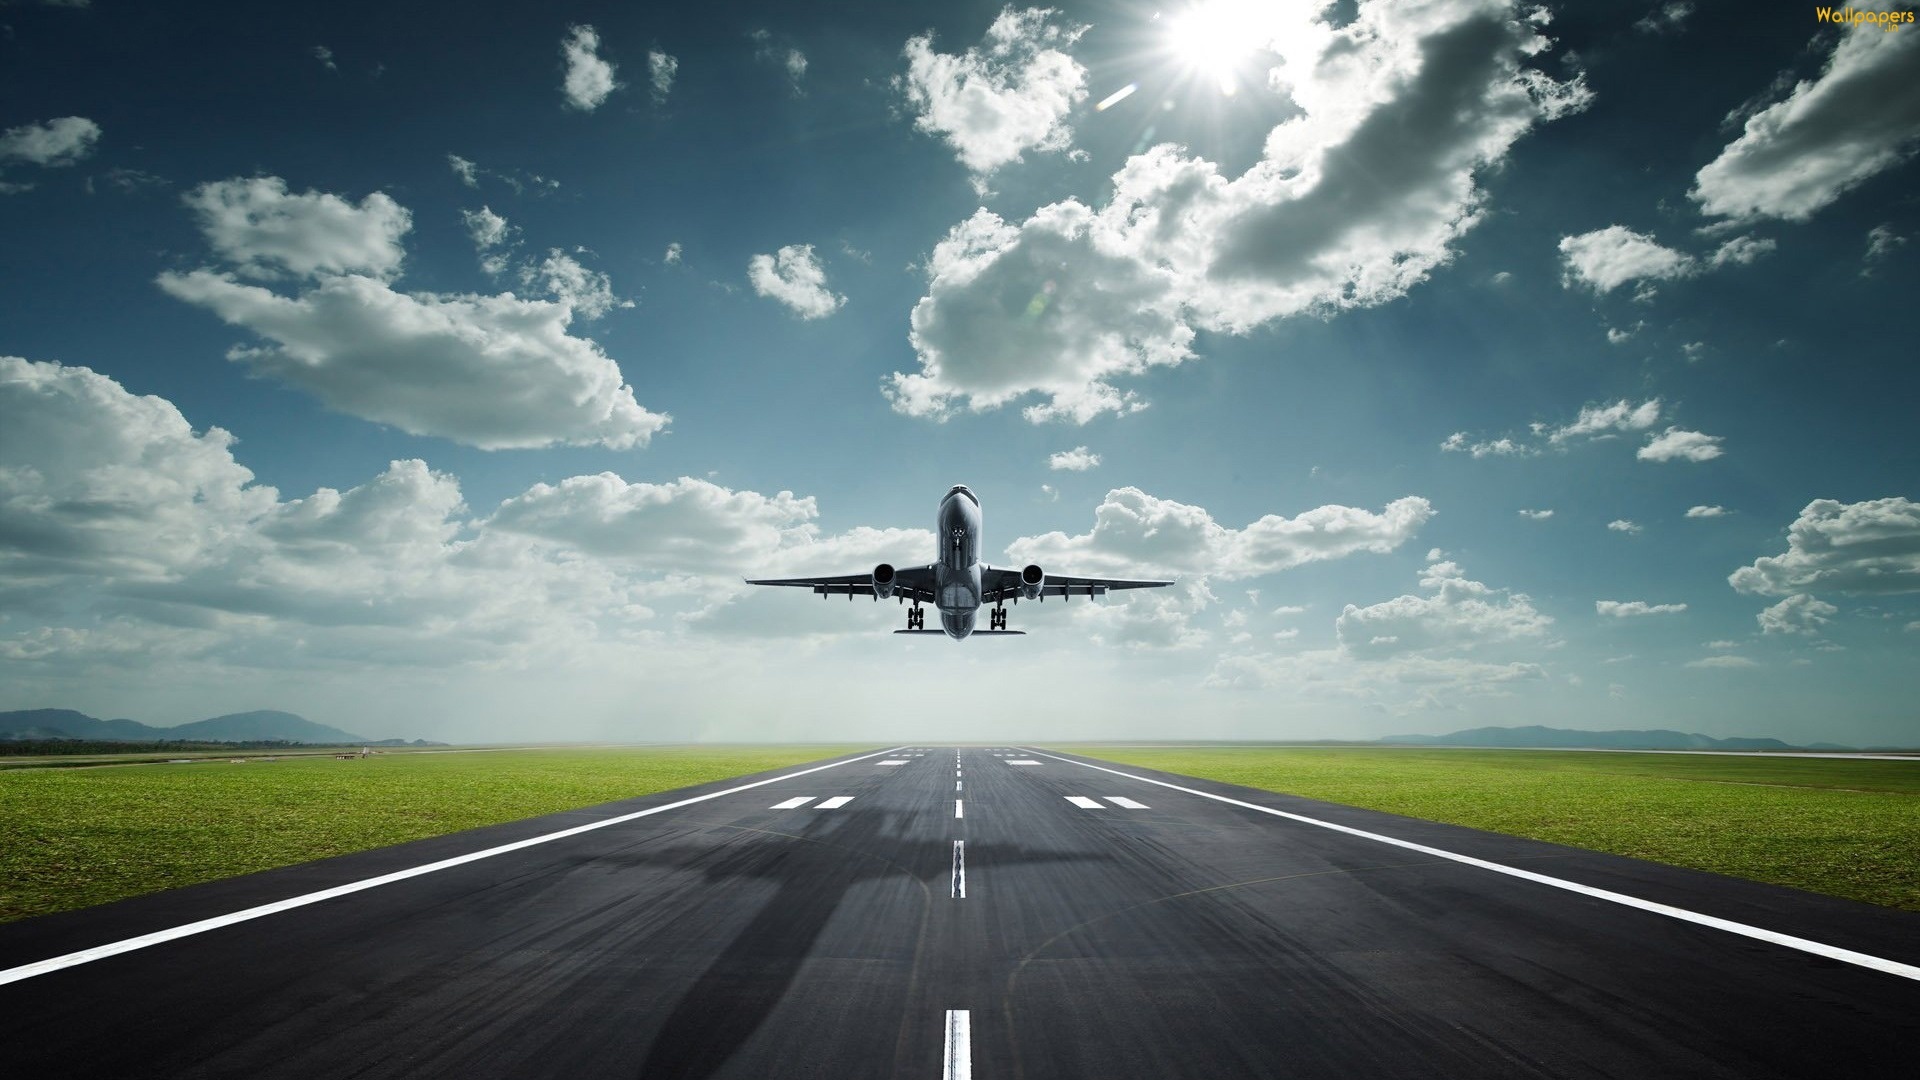
\includegraphics[height=\paperheight]{takeoff.jpg}
    }
    \begin{frame}
        \frametitle{Thank you for the attention}
        \begin{center}
        	\vskip 2cm
            \textbf{Thank you for the attention}
        \end{center}
    \end{frame}
    }

\end{document}
